\documentclass{article}

% Bibliography
\usepackage{natbib}
\bibpunct{(}{)}{;}{a}{}{;}

% Use 'It was found that A is B (Name 1234)' style
\setcitestyle{authoryear,open={},close={}}

% Affiliations
\usepackage{authblk}
\title{pirouette: the error BEAST2 makes in inferring a phylogeny}
\author[1]{Rich\`el J.C. Bilderbeek}
\author[1]{Giovanni Laudanno}
\author[1]{Rampal S. Etienne}
\affil[1]{Groningen Institute for Evolutionary Life Sciences, University of Groningen, Groningen, The Netherlands}

% Use double spacing
\usepackage{setspace}
\doublespacing

\usepackage{listings}
\usepackage{hyperref}
\usepackage{todonotes}
\usepackage{verbatim}
\usepackage{pgf}
\usepackage{bm}

% sidewaysfigure
\usepackage{rotating}

% Style of listings
% From http://r.789695.n4.nabble.com/How-to-nicely-display-R-code-with-the-LaTeX-package-listings-tp4648110.html
\usepackage{fancyvrb} 
\definecolor{codegreen}{rgb}{0,0.6,0}
\definecolor{codegray}{rgb}{0.5,0.5,0.5}
\definecolor{codepurple}{rgb}{0.58,0,0.82}
\definecolor{backcolor}{rgb}{0.95,0.95,0.92}
\lstdefinestyle{mystyle}{
  language=R,% set programming language
  basicstyle=\ttfamily\small,% basic font style
  commentstyle=\color{gray},% comment style
  % numbers=left,% display line numbers on the left side
  numberstyle=\scriptsize,% use small line numbers
  numbersep=10pt,% space between line numbers and code
  tabsize=2,% sizes of tabs
  showstringspaces=false,% do not replace spaces in strings by a certain character
  captionpos=b,% positioning of the caption below
  breaklines=true,% automatic line breaking
  escapeinside={(*}{*)},% escaping to LaTeX
  fancyvrb=true,% verbatim code is typset by listings
  extendedchars=false,% prohibit extended chars (chars of codes 128--255)
  alsoletter={.<-},% becomes a letter
  alsoother={$},% becomes other
  otherkeywords={!=, ~, $, \&, \%/\%, \%*\%, \%\%, <-, <<-, /},% other keywords
  deletekeywords={c}% remove keywords 
}
\lstset{style=mystyle}

% Adds numbered lines
\usepackage{lineno}
\linenumbers

% Rename 'Abstract' to 'Summary 
\usepackage[english]{babel}
\addto{\captionsenglish}{\renewcommand{\abstractname}{Summary}}

%comments
\newcommand{\giovanni}[1]{\textcolor{blue}{\textbf{[GL: #1]}}}
\newcommand{\richel}[1]{\textcolor{orange}{\textbf{[RB: #1]}}}

\begin{document}

\maketitle

\begin{abstract}

  \textbf{1. }
    BEAST2 is a popular Bayesian phylogenetics software tool,
    that takes an alignment and an inference model to create a
    posterior of jointly-estimated phylogenies and model parameter estimates.
    When a new macro-evolutionary diversification model is developed,
    a good first step is to measure the error BEAST2 makes, with its current set of inference models, on a known
    phylogeny derived from a new diversification mechanism. \\
  \textbf{2. }
    Here we present \verb;pirouette;, a free, libre and open-source R package that assesses the inference error BEAST2 makes based on a known/true 
    phylogeny. \\
  \textbf{3. }
    We describe \verb;pirouette;'s usage and the biological scientific
    question it can answer, including full examples. \\
  \textbf{4. }
    Last, we will discuss the results obtained by the examples. \\
\end{abstract}

{\bf Keywords:} computational biology, evolution, phylogenetics, BEAST2, pirouette, R

%%%%%%%%%%%%%%%%%%%%%%%%%%%%%%%%%%%%%%%%%%%%%%%%%%%%%%%%%%%%%%%%%%%%%%%%%%%%%%%%%%%%%%
\section{Introduction}
%%%%%%%%%%%%%%%%%%%%%%%%%%%%%%%%%%%%%%%%%%%%%%%%%%%%%%%%%%%%%%%%%%%%%%%%%%%%%%%%%%%%%%

The development of new powerful inference tools, 
such as BEAST [\cite{drummond2007beast}], MrBayes [\cite{huelsenbeck2001mrbayes}]
or RevBayes [\cite{hohna2016revbayes}], 
allows to build phylogenetic trees 
from genetic material extracted from extant organisms.
This has constituted an important step forward 
in our understanding on how species evolve.
Such tools have been increasingly exploited to hypothesize 
and test what the main drivers and modes for diversification are.

Since BEAST performs a bayesian analysis, it needs not only genetic data but also tree priors, describing how the diversification occur, to return posterior phylogenies.
BEAST works using standard tree priors like Yule or birth-death \giovanni{integrate this if necessary}.
The recent development of BEAST2 [\cite{bouckaert2014beast}] provides, unlike its predecessor, the possibility for third-party users to integrate its prior libraries with new ones. Many of these have been developed, in the form of likelihood diversification models: birth-death models that have rates that are 
constant [\cite{nee1994reconstructed}], 
time-dependent [\cite{nee1994reconstructed}, \cite{rabosky2008explosive}], 
diversity-dependent [\cite{etienne2011diversity}],
or can shift [the SLS model. Laudanno et al., in preparation].
There are birth death models in which speciation is a process that 
takes time [\cite{rosindell2010protracted}][\cite{etienne2012prolonging}],
can co-occur [Laudanno et al., in preparation],
dependent on a trait that is binary [\cite{maddison2007estimating}], 
has multiple states [\cite{fitzjohn2012diversitree}],
has a concealed state [\cite{beaulieu2016detecting}] 
or has multiple observed and concealed states [\cite{herrera2018detecting}]. 

\iffalse
Such models usually rely on the assumption 
that a particular diversification process 
can be explained mainly by a specific mechanism.
Such a mechanism is built into a likelihood function, 
which provides the probability that a phylogeny is realized 
from a given set of parameters.
Starting from a phylogeny, this likelihood is maximized
to infer the best estimates for the parameter values.
For such diversification models, it is a standard practice 
to measure how well parameters can be recovered in this way,
by simulating 'true' phylogenies from known parameters, then
measuring the parameters deduced by maximum likelihood. 
\fi

From a given phylogeny, the likelihood is maximized
to infer the best estimates for the parameter values.
For such  models, it is a standard practice to assess their performance on a controlled environment: this is done by simulating phylogenies from known parameters, then comparing the estimations obtained by maximum likelihood with the original parameters.

\richel{
  We should bridge this method with how pirouette does things differently;
  why the maximum likelihood does not apply in this context  
}
\giovanni{
I will try writing a first draft of this
}
 If the likelihood proves to be effective to describe the process, it can be implemented into BEAST2 as a new prior. Despite that it is still possible that already existing BEAST2 priors will perform well enough and, therefore, that the introduction of a new model is not necessary.

Diversification models are getting more complex over time. 
This is facilitated by the increase in computing power due to the advancement of technology.
Increased complexity made possible the exploration of new models 
encompassing mechanisms that are not yet considered by previous diversification models. 
An example of this is the multiple-birth model [Laudanno et al., in preparation],
that is the first model to allow simultaneous speciations to co-occur.

However, whenever a new model is proposed there is always a trade-off 
between the cost of increased complexity versus the benefits that it can provide.
In fact developing models can cost time, human and computational resources.
Therefore desirable models have to be able to disentangle 
the intrinsic complexity of a system, 
highlight the main reasons of its behaviour and avoid unnecessary complexity. 

For this reason we believe it is important to have techniques 
to quantitatively assess the advancement provided by the introduction of new models, 
in comparison to the existing ones.

To achieve this, one possible experiment is to simulate a phylogeny 
according to the mechanisms proposed by the new diversification model, 
then simulate its alignment and measure how well current inference models perform 
at retrieving the original phylogeny.
If this difference is small enough, current models apparently
suffice.

\verb;pirouette; is an R package that performs such an experiment,
and is built on \verb;babette; [Bilderbeek \& Etienne, 2018], 
which calls BEAST2 [\cite{bouckaert2014beast}]. 
With \verb;pirouette;, one
can easily measure the error made by Bayesian inference in recovering
any given phylogeny, helping us to evaluate the necessity of a new diversification model.
Once verified that the introduction of a new model is indeed beneficial,
\iffalse
Upon finding a diversification model is warranted, 
\fi
it can then be added to BEAST2's existing set of (birth-death and 
coalescent) models via the BEAST2 package system.

%%%%%%%%%%%%%%%%%%%%%%%%%%%%%%%%%%%%%%%%%%%%%%%%%%%%%%%%%%%%%%%%%%%%%%%%%%%%%%%%%%%%%%
\section{Description}
%%%%%%%%%%%%%%%%%%%%%%%%%%%%%%%%%%%%%%%%%%%%%%%%%%%%%%%%%%%%%%%%%%%%%%%%%%%%%%%%%%%%%%

\verb;pirouette; is written in the R programming language (\cite{R}).

\iffalse
The goal of \verb;pirouette; is to measure the inference error BEAST2
makes from a given reconstructed phylogeny, within the context of
a simulation study on a (possibly new) diversification model. Such
a study will typically construct phylogenies for different combinations of the diversification model's parameters, to assess under which scenarios the error made by BEAST2 cannot be ignored anymore. 
Such a study needs to be done on, there need be many replicates.
\fi

The goal of \verb;pirouette; is to measure the inference error made by BEAST2 from a given reconstructed phylogeny, which has been simulated according to a (possibly new) diversification model.
To do that the full procedure would be to simulate a great number of phylogenies for different combinations of the diversification model's parameters, to assess under which scenarios the error made by BEAST2 cannot be ignored anymore. 

To be able to explain how \verb;pirouette; measures the inference error
BEAST2 makes, we first give two definitions of what
we mean by a generative model and by an inference model: 
a generative model is a combination of site model, clock model and tree prior,
used to simulate alignments. An inference model is a combination of 
site model, clock model, tree prior, an optional node calibration prior
and setup of the Markov chain Monte Carlo (MCMC) algorithm, 
used to produce a posterior. Node calibration priors, called 'most
recent common ancestor' (MRCA) priors within BEAST2, allow to create a time-calibrated phylogeny, by specifying a normal distribution around an expected time when the ancestors of two or more taxa diversified. 

\subsection{pirouette's pipeline}

\begin{sidewaysfigure}
  \centering
  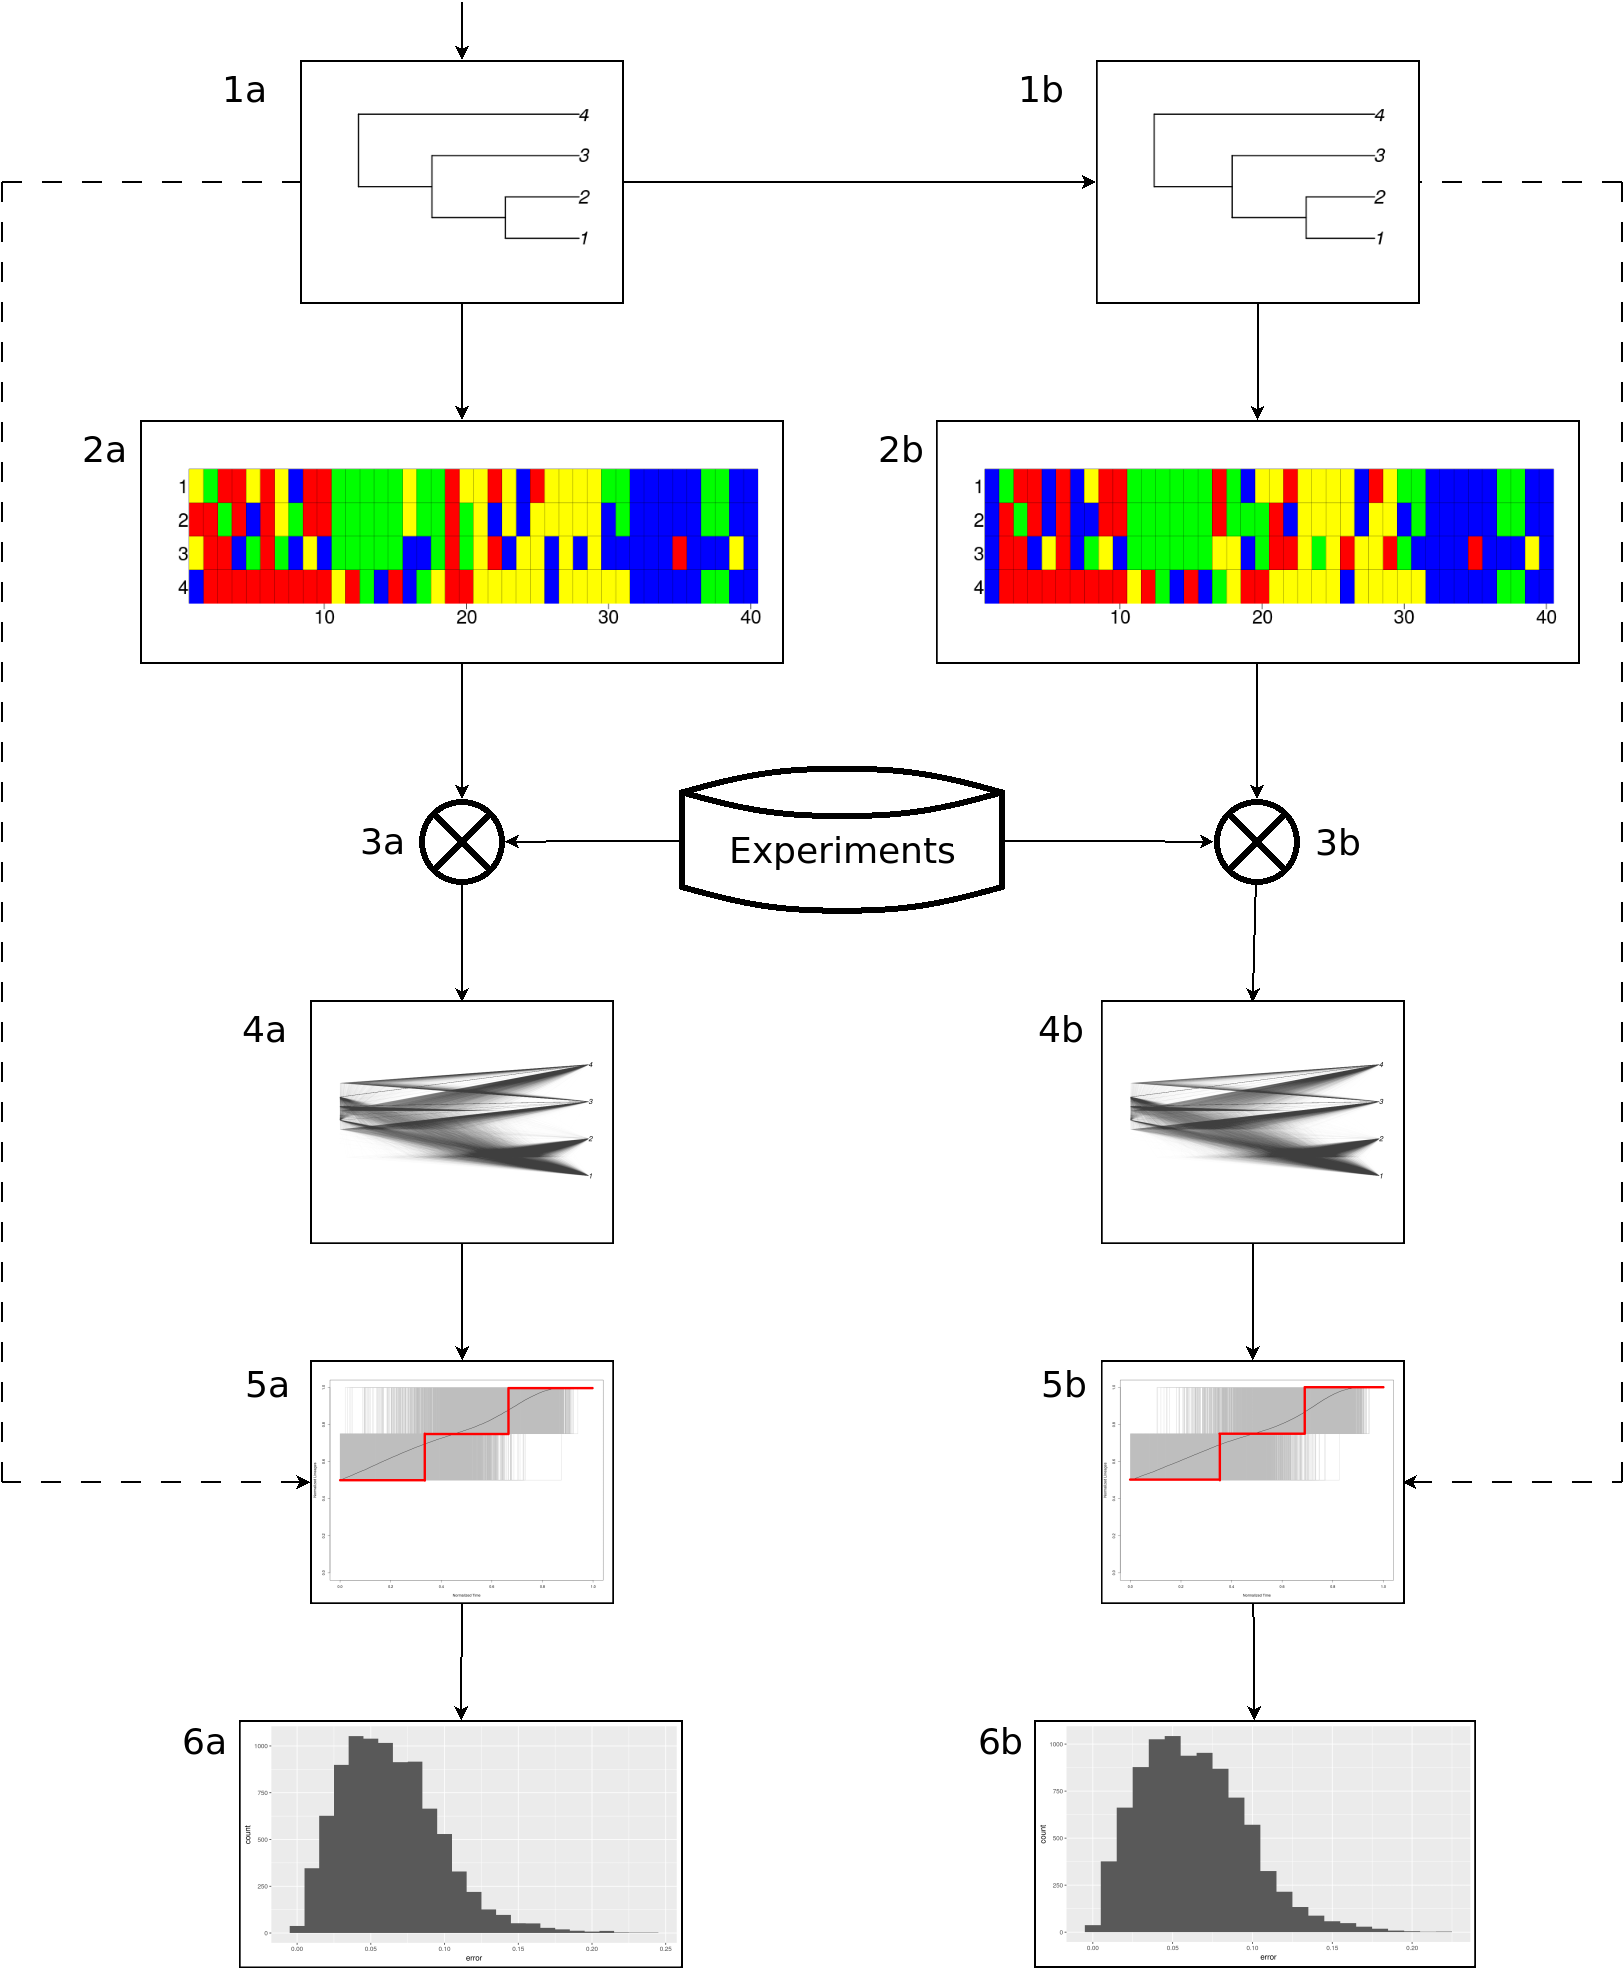
\includegraphics[width=\textwidth]{workflow.png}
  \caption{
  pirouette pipeline
  \giovanni{
  see \texttt{https://github.com/richelbilderbeek/pirouette\_article/issues/9}
  }
  }
  \label{fig:pipeline}
\end{sidewaysfigure}

The pipeline is summarized by the following steps, which will be described in detail below:
\begin{enumerate}
    \item from a given phylogeny an alignment is simulated;
    \item from the alignment an inference model is chosen;
    \item the alignment is used as BEAST2 input to infer a posterior distribution of phylogenies;
    \item posterior phylogenies are compared with the given original phylogeny to estimate the error we make. The higher the match, the lower the error;
\end{enumerate}
The pipeline is visualized in Fig.~\ref{fig:pipeline}.
There is also the option to generate a 'twin tree',
that goes through the same pipeline.

The first step simulates a DNA alignment from the given phylogeny.
One can specify a DNA sequence
of any length at the root of the phylogeny, a DNA mutation rate, a
site (i.e. nucleotide substitution) model, 
a clock model, a random number generator (RNG) seed and a location
where the alignment is saved to. This step is relatively fast, but longer
DNA alignments will noticeably slow down the inference step.

The second step selects an inference model, using the alignment.
The user can specify whether to use the generative model or select the best model
from a set of inference models. 
When selecting the generative model,
the site and clock model used in the alignment simulation are used
in the inference. Because the given phylogeny (on which the alignment is based)
may have followed any tree prior (i.e. speciation model), the user needs
to specify which tree prior is used in the inference. 
When selecting for the best
model, the alignment is used to find the inference model that has the
highest evidence (i.e. marginal likelihood) from a set of candidate inference models.
The evidence of an inference model is estimated using a nested sampling (NS)
approach, as described in \cite{maturana2018model}. The nested sampling is
performed by \verb;mcbette; [\cite{mcbette}], that calls the 'NS' BEAST2 package. 
Using BEAST2 packages (in a scripted way) can only be done under Linux and Mac; 
inference model selection is not available on Windows.

The third step infers a Bayesian posterior from the simulated alignment,
using the inference model(s) selected in the previous step. The user
can specify the additional parameters needed for the BEAST2 run, which
are the Markov-Chain Monte Carlo (MCMC) setup, 
an optional Most Recent Common Ancestor (MRCA) \giovanni{MRCA has been already been defined. It is therefore possible to use the acronym only, if you want} prior and an RNG seed.
The MCMC setup determines the number of posterior trees sampled.
An MRCA prior allows the inferred phylogeny to have a dated crown age.

The fourth step measures the inference error, using the phylogenies in the
Bayesian posterior. These phylogenies are compared to the given
original phylogeny using an error statistic, which is the nLTT 
statistic (\cite{janzen2015approximate}) by default,
but also a custom error statistic is supplied, based
on the absolute difference in the gamma statistic [\cite{pybus2000testing}]. 
Additionally, the user can specify the
proportion of posterior phylogenies to 
discard (i.e. the burn-in), throwing away the first $10\%$
of all phylogenies by default. This burn-in is used to discard
the part of the MCMC chain that has not yet converged to a
representative part of the state space.

\subsection{Twin tree}

\iffalse
An optional step is to generate a 'twin tree', that will be
analyzed in the same way as the true tree.
The twin tree has the same topology as the given phylogeny, yet its branch lengths follow the same distribution as a Yule (pure-birth) or (constant rate) birth-death tree prior \giovanni{let's revise this after we meet Rampal and define how a twin tree should be created}.
The use of such a twin tree, is to assess the minimum level of noise (i.e. error) BEAST2 makes when the input (the twin phylogeny) has an ideal branch length distribution.
\fi

An optional step is to generate a 'twin tree', that will be
analyzed in the same way as the true tree.
The twin tree has the same topology as the given phylogeny, yet its branching times are simulated according to the tree prior used by BEAST2 to produce a posterior.
The goal of this procedure is to generate a tree to use as a control for the main experiment.
The procedure to generate a twin tree is the following:

From the given phylogeny we maximize a birth-death likelihood [\cite{nee1994reconstructed}] to infer the standard birth-death rates, namely speciation rate $\lambda$ and extinction rate $\mu$.

We use $\lambda$ and $\mu$ to simulate a new birth-death tree, conditioned on having the same number of tips as the original tree. We store its branching times.

We then combine such branching times with the original tree's topology to obtain the twin tree.

%%%%%%%%%%%%%%%%%%%%%%%%%%%%%%%%%%%%%%%%%%%%%%%%%%%%%%%%%%%%%%%%%%%%%%%%%%%%%%%%%%%%%%
\section{Installation}
%%%%%%%%%%%%%%%%%%%%%%%%%%%%%%%%%%%%%%%%%%%%%%%%%%%%%%%%%%%%%%%%%%%%%%%%%%%%%%%%%%%%%%

\verb;pirouette; can be installed easily from CRAN:

\begin{lstlisting}[language=R, floatplacement=H, frame=single]
install.packages("pirouette")
\end{lstlisting}

For the most up-to-date version, 
one can download and install the package from \verb;pirouette;'s GitHub repository:

\begin{lstlisting}[language=R, floatplacement=H, frame=single]
usethis::install_github("richelbilderbeek/pirouette")
\end{lstlisting}

To start using \verb;pirouette;, load its functions in the global namespace first:

\begin{lstlisting}[language=R, floatplacement=H, frame=single]
library(pirouette)
\end{lstlisting}
Because \verb;pirouette; calls BEAST2, BEAST2 must be installed. 
This can be done from within R, using:

\begin{lstlisting}[language=R, floatplacement=H, frame=single]
install_beast2()
\end{lstlisting}
For the option to select inference models,
\verb;pirouette; uses the "NS" BEAST2 package [\cite{maturana2018model}].
It can be installed from within R, using:

\begin{lstlisting}[language=R, floatplacement=H, frame=single]
install_beast2_pkg("NS")
\end{lstlisting}

%%%%%%%%%%%%%%%%%%%%%%%%%%%%%%%%%%%%%%%%%%%%%%%%%%%%%%%%%%%%%%%%%%%%%%%%%%%%%%%%%%%%%%
\section{Usage: first research question}
%%%%%%%%%%%%%%%%%%%%%%%%%%%%%%%%%%%%%%%%%%%%%%%%%%%%%%%%%%%%%%%%%%%%%%%%%%%%%%%%%%%%%%

A first research question that \verb;pirouette; answers is:
"What is the error BEAST2 makes \giovanni{I would prefer "the error made by BEAST2" in place of "the error BEAST2 makes"} from a phylogeny using the same diversification model as it was generated by?"

\iffalse
We start with an idealised \giovanni{the word idealized cannot be used unless we specify what it means.} Yule (pure-birth) tree 
with five taxa and a crown age of ten.
By idealized, we mean a phylogeny that is easiest to recover
by the Bayesian inference. A phylogeny that is easy to recover has
the most common branch length distribution imaginable. We
use an idealised tree, as we want to measure the baseline noise; that is, the lowest error that BEAST2 can possibly make.
\fi

We start with a Yule (pure-birth) tree with five taxa and a crown age of ten.

\begin{lstlisting}[
    language=R, floatplacement=H, frame=single, 
    label = {lst:create_ideal_tree}, 
    caption = {Create an ideal tree}
  ]
phylogeny <- create_ideal_tree(n_taxa = 5, crown_age = 10)
\end{lstlisting}

\begin{figure}[h]
  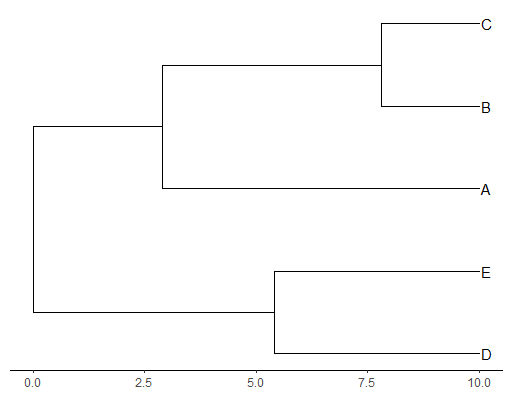
\includegraphics[width=\textwidth]{figure_bd.png}
  \caption{The ideal tree, as created by listing \ref{lst:create_ideal_tree}}
\end{figure}

The first step in \verb;pirouette; is to simulate a DNA alignment from the given phylogeny. To do so, we must specify the DNA root sequence and a mutation rate. In this example, the DNA root sequence consists out of four block of 250 nucleotides each, where the per-nucleotide mutation rate is 0.1 mutations per unit time.

\begin{lstlisting}[
    language=R,
    floatplacement=H, frame=single,
    label = {lst:create_alignment}, 
    caption = {Create an alignment}
  ]
alignment_params <- create_alignment_params(
  root_sequence = create_blocked_dna(length = 1000),
  mutation_rate = 0.1
)
\end{lstlisting}

By default, an alignment is created using a Jukes-Cantor (JC) site model
and a strict clock model. A JC site model assumes that mutation rates from any nucleotide to any other are equal and constant. A strict clock model assumes that the mutation rates of all species are equal and constant.
Due to this, we state that the generative model for the alignment is
a JC site model and a strict clock model.

\iffalse
In the second step we state our experiments. In this context, we
define an experiment as a combination of an inference model
and the conditions under which a Bayesian inference is executed.
Within this example, we specify that our experiment uses the
generative model, will always be run and we ignore the evidence for our model,
for the inference model that is also the generative model (using a
JC site model, strict clock model and Yule tree prior).
\fi

In the second step we state our experiments. In this context, we
define an experiment as a combination of an inference model
and the conditions under which a Bayesian inference is executed.
Within this example, we specify that our experiment uses the
generative model (which means that the inference model will be a combination of JC site model, strict clock model and Yule tree prior), will always be run and we don't need to measure the evidence for our model.

\begin{table}
  \begin{tabular}{ | c | c | c | l | }
    \hline
    \textbf{model type} & \textbf{run if} & \textbf{measure evidence} & \textbf{inference model} \\ 
    \hline
    generative & always & no & JC, strict, Yule \\
    \hline
  \end{tabular}
  \caption{
    Experimental setup to answer the first research question.
    JC: Jukes-Cantor site model.
    strict: strict clock model.
    Yule: Yule (pure-birth) tree prior.
  }
  \label{tbl:RQ1}
\end{table}

Due to sensible defaults, specifying this
results in:

\begin{lstlisting}[
  language=R, 
  floatplacement=H, frame=single,
  label = {lst:create_generative_experiment},
  caption = {
    Create a default experiment, as described in Table~\ref{tbl:RQ1}.
  }
]
experiments <- list(create_experiment())
\end{lstlisting}

All the \verb;pirouette; arguments are bundled
and checked by \verb;create_pir_params;:

\begin{lstlisting}[language=R, floatplacement=H, frame=single]
pir_params <- create_pir_params(
  alignment_params = alignment_params,
  experiments = experiments
)
\end{lstlisting}

Running the experiment:

\begin{lstlisting}[language=R, floatplacement=H, frame=single]
errors <- pir_run(
  phylogeny,
  pir_params = pir_params
)
\end{lstlisting}

\verb;pirouette; has a nice plotting function:

\begin{lstlisting}[language=R, floatplacement=H, frame=single]
pir_plot(errors)
\end{lstlisting}

The resulting figure is shown in figure \ref{fig:example_1}.

\begin{figure}[h]
  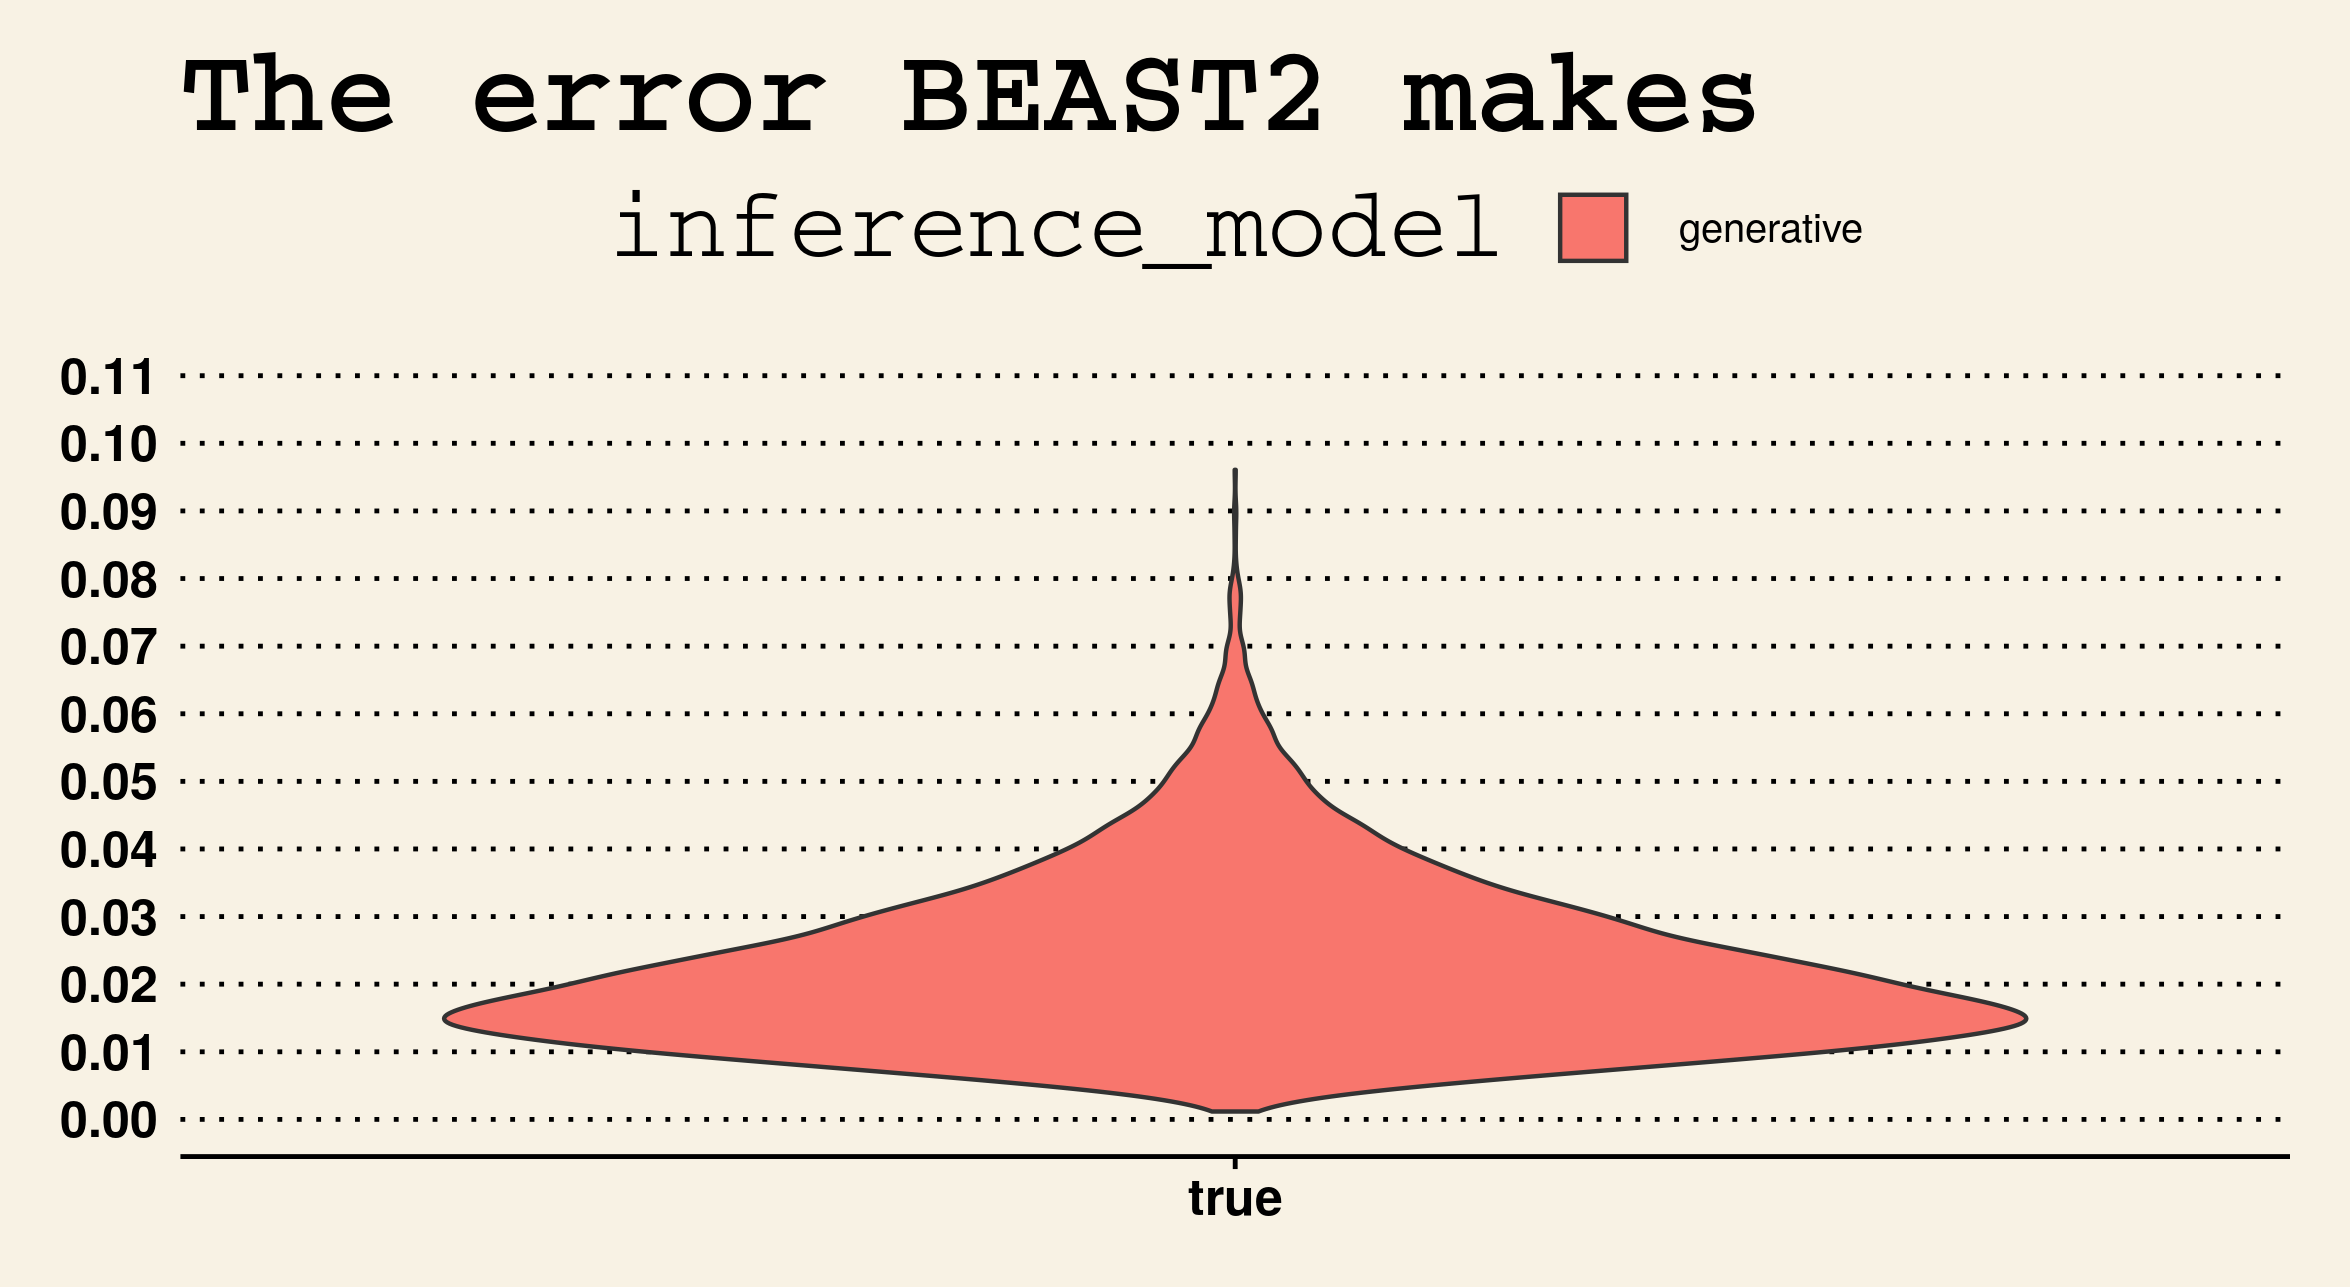
\includegraphics[width=\textwidth]{figure_example_1.png}
  \caption{
    The error BEAST2 makes from a phylogeny 
    when the generative and inference model are the same.
  }
  \label{fig:example_1}
\end{figure}

%%%%%%%%%%%%%%%%%%%%%%%%%%%%%%%%%%%%%%%%%%%%%%%%%%%%%%%%%%%%%%%%%%%%%%%%%%%%%%%%%%%%%%
\section{Usage: second research question}
%%%%%%%%%%%%%%%%%%%%%%%%%%%%%%%%%%%%%%%%%%%%%%%%%%%%%%%%%%%%%%%%%%%%%%%%%%%%%%%%%%%%%%

A second research question that \verb;pirouette; answers, is:
"What is the error BEAST2 makes from a phylogeny when
picking the best inference model?"

Here we start with a tree generated from an unknown 
diversification model, that has four taxa and a crown age of five:

\begin{lstlisting}[
  language=R, 
  floatplacement=H, 
  frame=single, 
  label = {lst:unknown_phylogeny},
  caption = A phylogeny generated by an unknown diversification model
]
phylogeny <- ape::read.tree(text = "((A:4, B:4):1, (C:4, D:4):1);")
\end{lstlisting}

The first step in \verb;pirouette; is to simulate a DNA alignment from the given phylogeny. We will re-use the alignment parameters of the previous example as shown in listing \ref{lst:create_alignment}.

\begin{table}
  \begin{tabular}{ | c | c | c | l | }
    \hline
    \textbf{model type} & \textbf{run if} & \textbf{measure evidence} & \textbf{inference model} \\ 
    \hline
    candidate & best candidate & yes & JC, strict, Yule \\
    candidate & best candidate & yes & JC, strict, BD \\
    ...       & ...            & ... & ... \\
    candidate & best candidate & yes & GTR, RLN, CCP \\
    candidate & best candidate & yes & GTR, RLN, CEP \\
    \hline
  \end{tabular}
  \caption{
    Experimental setup to answer the second research question.
    JC: Jukes-Cantor site model.
    strict: strict clock model.
    Yule: Yule (pure-birth) tree prior.
    BD: birth-death tree prior.
    GTR: GTR site model.
    RLN: relaxed log-normal clock model.
    CCP: coalescent constant-population tree prior.
    CEP: coalescent exponential-population tree prior.
  }
\end{table}

In the second step we state our experiments. 
Within this example, all our experiments are candidates,
run only if it is the best candidate, the evidence is measured (ignoring
this will give a helpful error) and we use the full arsenal of 
40 inference models, which are all combinations of 4 site 
models, 2 clock models and 5 tree priors.

\begin{lstlisting}[language=R, floatplacement=H, frame=single]
experiments <- create_all_experiments()
\end{lstlisting}

Also here, the third (the BEAST2 inference) and fourth (measuring the error)
steps have sensible defaults, and we are not
interested in using a twin tree. We can create the complete
\verb;pirouette; parameter set (again) like this:

\begin{lstlisting}[language=R, floatplacement=H, frame=single]
pir_params <- create_pir_params(
  alignment_params = alignment_params,
  experiments = experiments
)
\end{lstlisting}

Running the experiment:

\begin{lstlisting}[language=R, floatplacement=H, frame=single]
errors <- pir_run(
  phylogeny,
  pir_params = pir_params
)
\end{lstlisting}

Again, showing the results:

\begin{lstlisting}[language=R, floatplacement=H, frame=single]
pir_plot(errors)
\end{lstlisting}

The resulting figure is shown in figure \ref{fig:example_2}.

\giovanni{After having explained that we are going to use as candidates all the possible inference models, it comes natural to wonder what is the best inference model selected by marginal likelihoods. It could be nice maybe, adding the name in the lengend on top-right, in place of the generic "candidate" word. It could be also nice to add it in the caption and/or in the main text.}

\begin{figure}[h]
  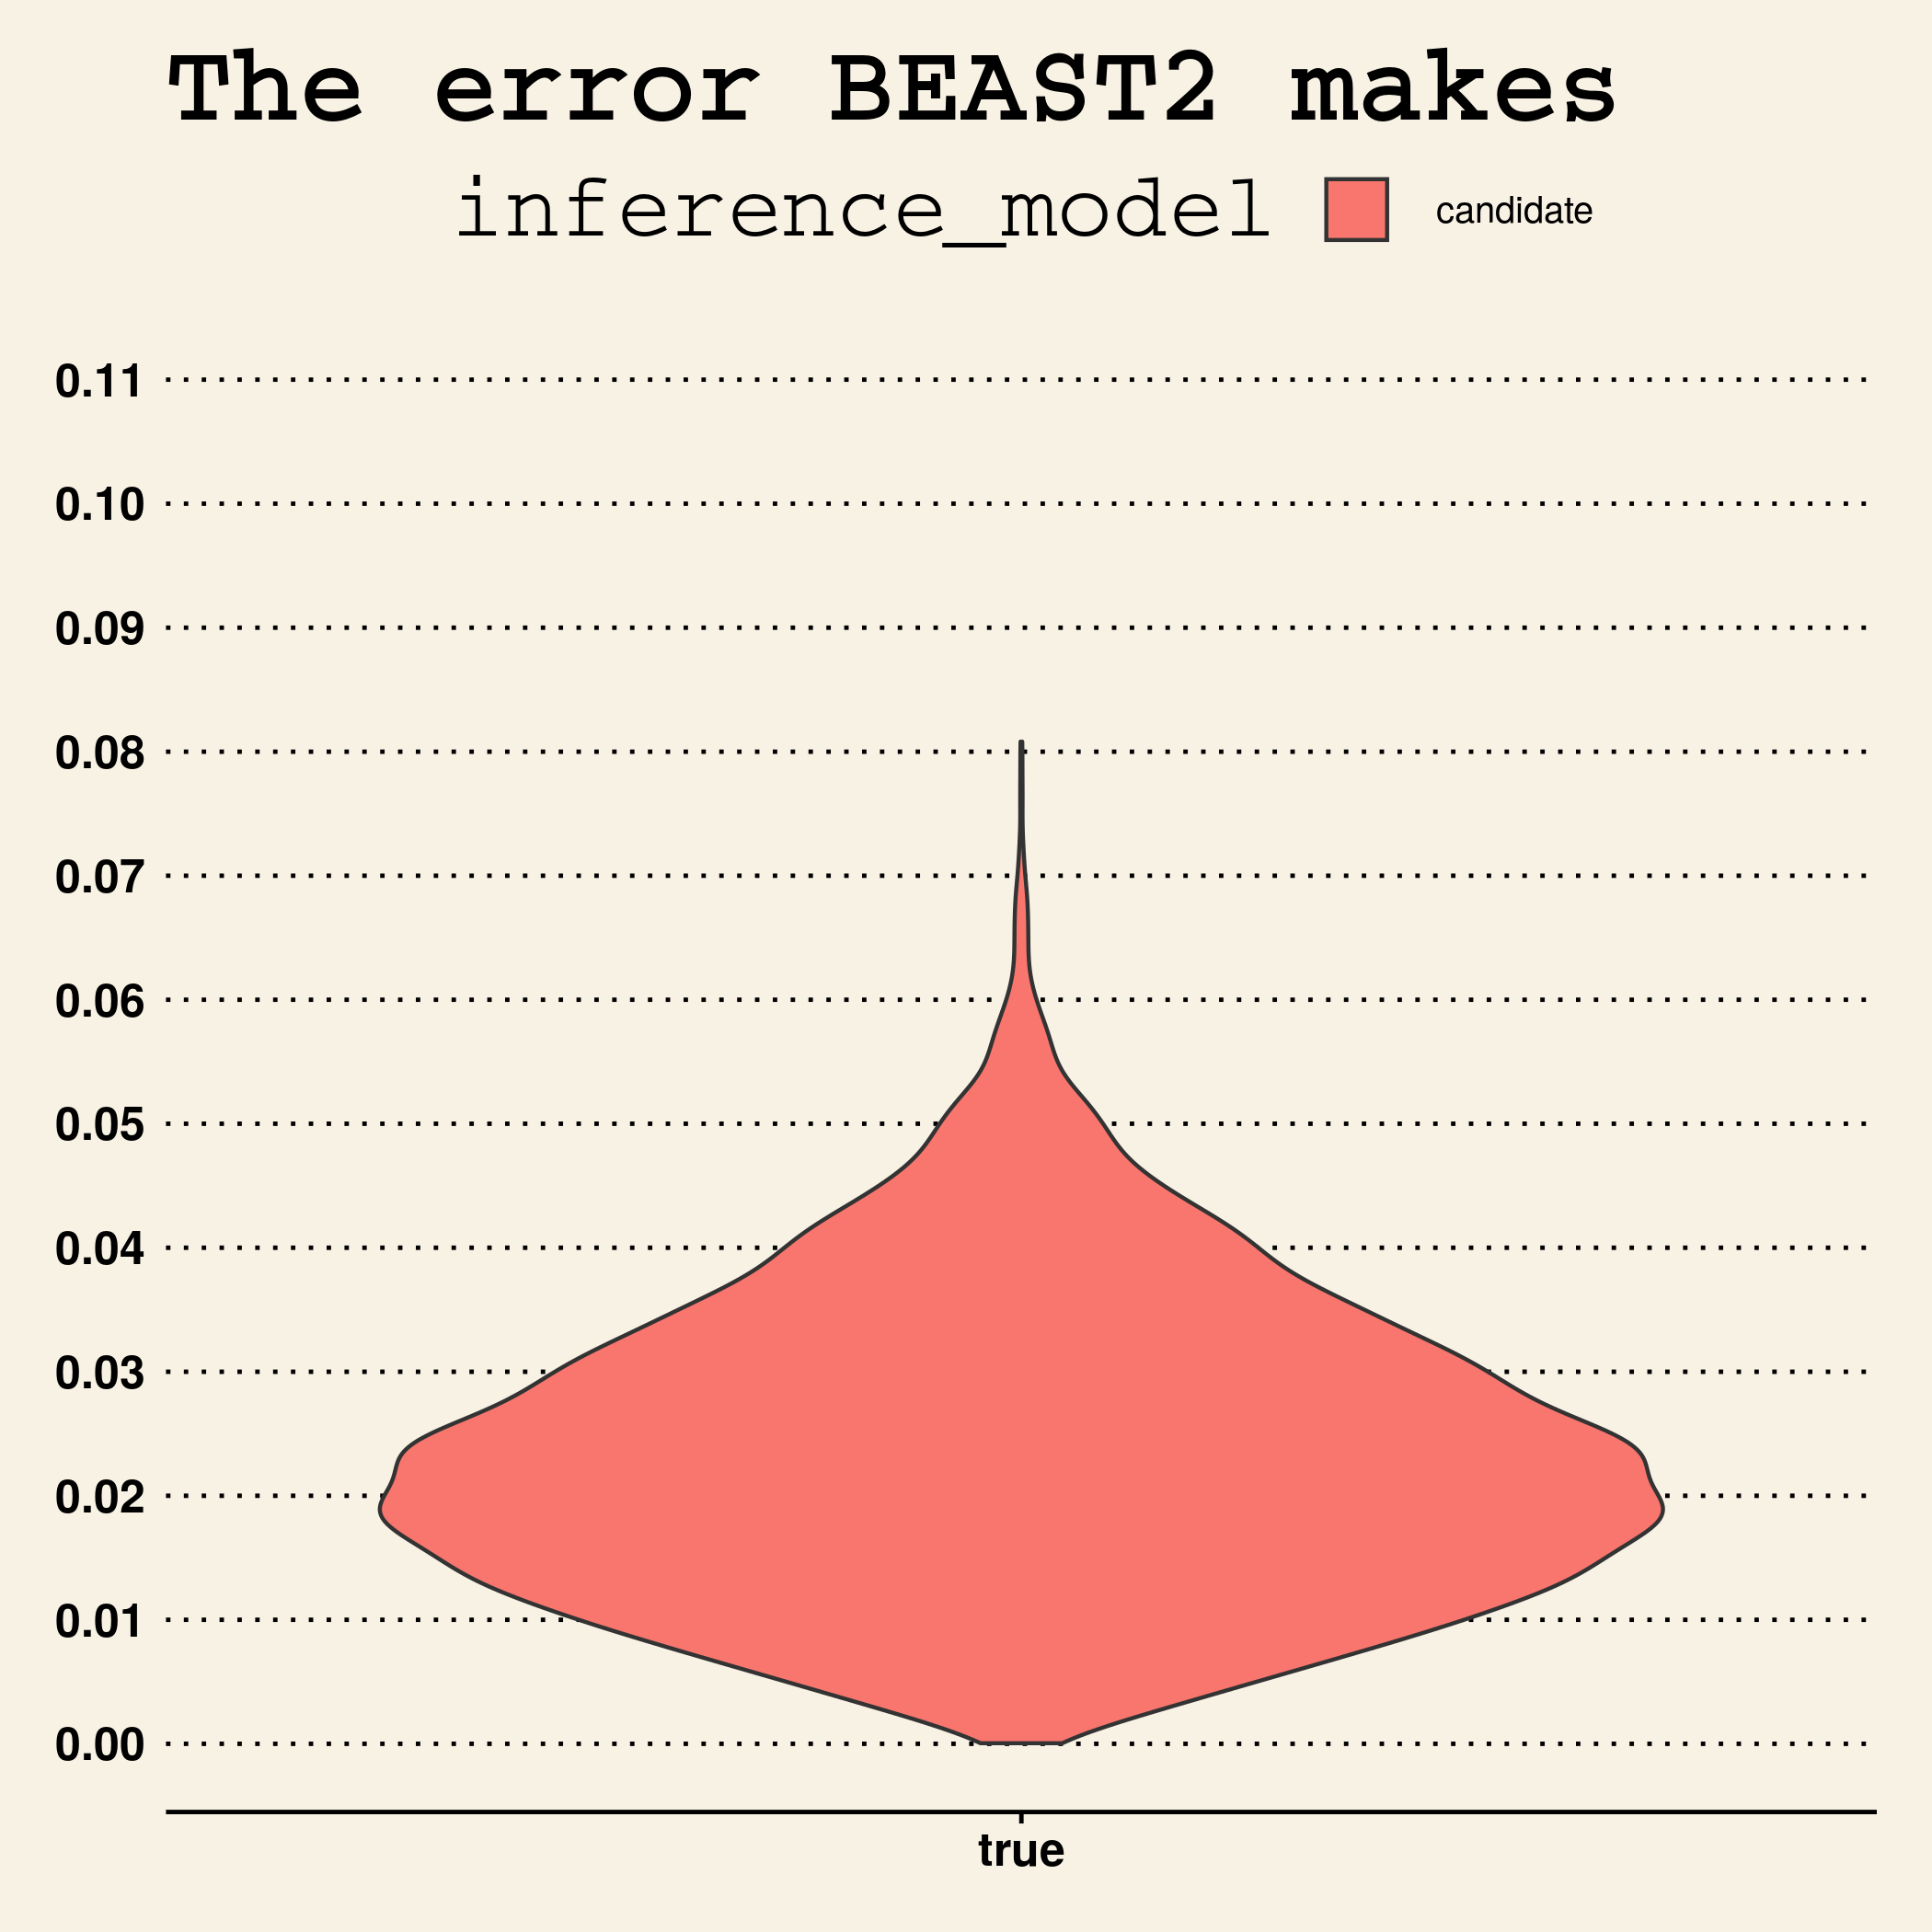
\includegraphics[width=\textwidth]{figure_example_2.png}
  \caption{
    The error BEAST2 makes from a phylogeny when
    picking the best inference model
  }
  \label{fig:example_2}
\end{figure}

%%%%%%%%%%%%%%%%%%%%%%%%%%%%%%%%%%%%%%%%%%%%%%%%%%%%%%%%%%%%%%%%%%%%%%%%%%%%%%%%%%%%%%
\section{Usage: third research question}
%%%%%%%%%%%%%%%%%%%%%%%%%%%%%%%%%%%%%%%%%%%%%%%%%%%%%%%%%%%%%%%%%%%%%%%%%%%%%%%%%%%%%%

A third research question that \verb;pirouette; answers is:
"What is the error BEAST2 makes from a phylogeny, 
when hand-picking an inference model, compared to the background noise?"

The following settings are the same as in the previous section:
phylogeny (listing \ref{lst:unknown_phylogeny}), 
alignment parameters (listing \ref{lst:create_alignment}), 
experiments (listing \ref{lst:create_generative_experiment}),
BEAST2 inference and error measuring parameters.

\iffalse
This time, we are interested in creating a twin tree. A twin tree
has the same topology as the given tree, yet its branch lengths follow
a distribution as such that the BEAST2 error will be 
close to \richel{'close to' is a bit weasly, but currently it is true}
its minimal error.
\fi

This time, we are interested in creating a twin tree. A twin tree
has the same topology as the given tree, yet its branching times are simulated according to the tree prior used by BEAST2 to produce a posterior. Since there is coherence between the inference model and the generative model, we expect BEAST2 to produce a posterior of phylogenies clearly more similar to the original one. We intend to use this as a control experiment.

Creating a twinning parameter is easy, as it has sensible default settings:

\begin{lstlisting}[language=R, floatplacement=H, frame=single]
twinning_params <- create_twinning_params()
\end{lstlisting}

We can now measure the errors made by BEAST2 when inferring the given phylogeny versus the error it makes when the same procedure is applied to the twin tree.

All the \verb;pirouette; arguments are bundled and checked by \verb;create_pir_params;:

\begin{lstlisting}[language=R, floatplacement=H, frame=single]
pir_params <- create_pir_params(
  alignment_params = alignment_params,
  experiments = experiments,
  twinning_params = twinning_params
)
\end{lstlisting}

Running:

\begin{lstlisting}[language=R, floatplacement=H, frame=single]
errors <- pir_run(
  phylogeny,
  pir_params = pir_params
)
\end{lstlisting}

Again, showing the results:

\begin{lstlisting}[language=R, floatplacement=H, frame=single]
pir_plot(errors)
\end{lstlisting}

The resulting figure is shown in figure \ref{fig:example_3}

\begin{figure}[h]
  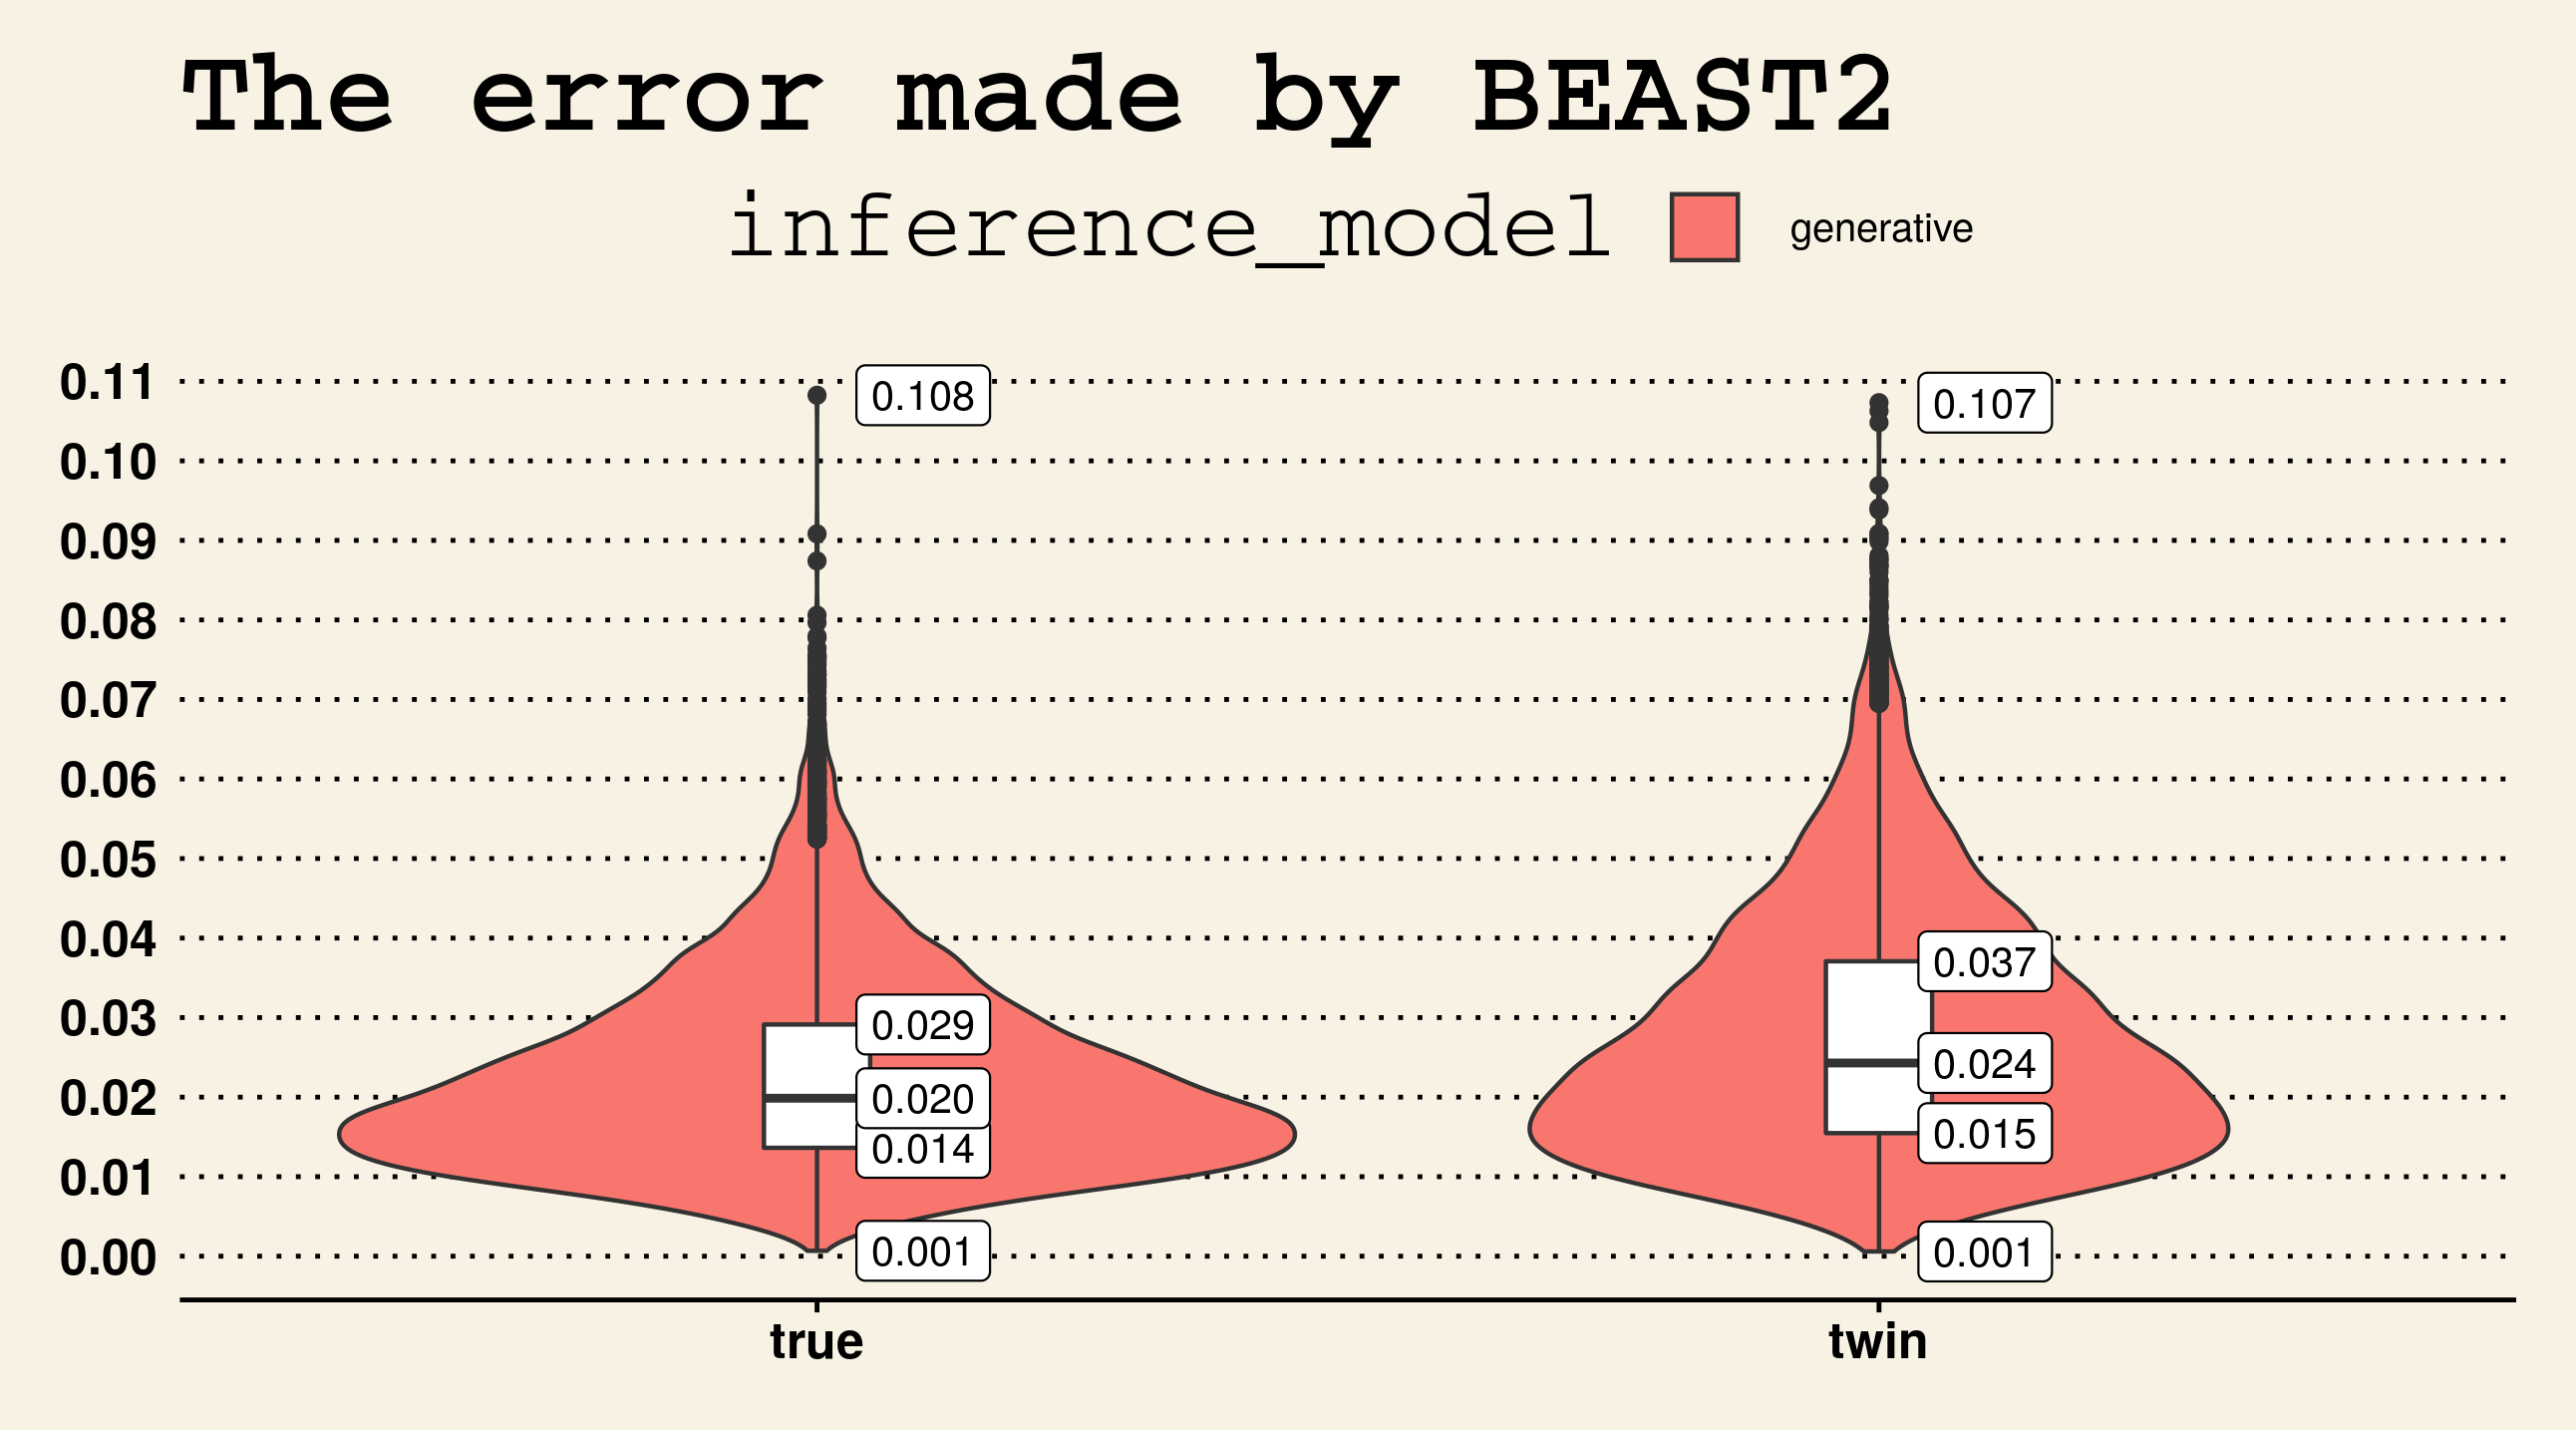
\includegraphics[width=\textwidth]{figure_example_3.png}
  \caption{
    The error BEAST2 makes from a phylogeny picking the best inference model versus the control.
    Here, the twin column shows the error BEAST2 makes starting from the original tree versus the twin. 
  }
  \label{fig:example_3}
\end{figure}

\iffalse
The error BEAST2 makes from a phylogeny 
picking the best inference model, compared to the background noise.
Here, the twin column shows the error BEAST2 makes on an idealized
tree, to measure the noise, which is the minimal error. 
\fi

%%%%%%%%%%%%%%%%%%%%%%%%%%%%%%%%%%%%%%%%%%%%%%%%%%%%%%%%%%%%%%%%%%%%%%%%%%%%%%%%%%%%%%
\section{Other examples}
%%%%%%%%%%%%%%%%%%%%%%%%%%%%%%%%%%%%%%%%%%%%%%%%%%%%%%%%%%%%%%%%%%%%%%%%%%%%%%%%%%%%%%

There are many other examples that can be found in the \verb;pirouette; 
documentation.

%%%%%%%%%%%%%%%%%%%%%%%%%%%%%%%%%%%%%%%%%%%%%%%%%%%%%%%%%%%%%%%%%%%%%%%%%%%%%%%%%%%%%%
\begin{table}[h]
\centering
\begin{tabular}{ | l | l | }
\hline
\textbf{Name} & \textbf{Description} \\
\hline
\verb;pir_run; & Run \verb;pirouette; \\
\verb;create_pir_params; & Create the \verb;pirouette; parameters \\
\hline
\verb;create_alignment_params; & Create the alignment parameters \\
\verb;create_twinning_params; & Create the twinning parameters \\
\verb;create_experiment; & Create one experiment \\
\verb;create_error_measure_params; & Create the error measurement parameters \\
\hline
\end{tabular}
\caption{pirouette's main functions}
\label{tab:functions}
\end{table}
%%%%%%%%%%%%%%%%%%%%%%%%%%%%%%%%%%%%%%%%%%%%%%%%%%%%%%%%%%%%%%%%%%%%%%%%%%%%%%%%%%%%%%

%%%%%%%%%%%%%%%%%%%%%%%%%%%%%%%%%%%%%%%%%%%%%%%%%%%%%%%%%%%%%%%%%%%%%%%%%%%%%%%%%%%%%%
\section{Discussion}
%%%%%%%%%%%%%%%%%%%%%%%%%%%%%%%%%%%%%%%%%%%%%%%%%%%%%%%%%%%%%%%%%%%%%%%%%%%%%%%%%%%%%%

Here we discuss how to interpret the results of \verb;pirouette;.
Figure \ref{fig:example_1} shows that the generative model 
gives an error distribution with a highest density \giovanni{probably "median" is a better word} at 0.02 \giovanni{I would increase the precision to the second significative digit, e.g. 0.017},
where the range of errors (in this case, the nLTT statistic) is from 0.0 to 1.0 \giovanni{providing standard deviation could be a better choice}.
The range of errors goes from 0.0 to 0.27 \giovanni{this is contrast with the last sentence}. As we know the generative model, this error distribution is the minimum noise that BEAST2 produces for this generative model.
\richel{Show effective sample size}

Figure \ref{fig:example_2} \giovanni{same as RQ1} shows that the best candidate model gives an error distribution with a highest density at 0.02, where the range of errors (in this case, the nLTT statistic) is from 0.0 to 1.0. The range of errors goes from 0.0 to 0.08. 
\richel{Describe and show evidences for the candidate model}
\richel{Describe and show the best candidate model}
This means that it is rational to use this inference model to 
infer a posterior phylogeny distribution, 
as is done by \verb;pirouette;.
\richel{Show effective sample size}
\richel{Show posterior phylogenies as densitree}

Figure \ref{fig:example_3} \giovanni{same as RQ1} shows that the hand-picked model gives an error distribution with a highest density at 0.018, with a range from 0.0 to 0.1.
The twin tree has an error distribution with a highest density at 0.019,
with a range from 0.0 to 0.11, which is the noise caused by the tree prior. \giovanni{I am still wondering if "noise" is the right term to use here. I still don't have a precise opinion on that. The problem is that for me it's a bit hard to interpret this without a distribution...}
As there is little difference between the true and twin tree,
the (unknown) diversification model has little impact on the error
BEAST2 makes, hinting that the constant-rate birth-death model is
sufficiently good enough to explain the true phylogeny. 
The diversification model apparently has minor impact and need not to be
added to BEAST2.

\giovanni{since you refer, for every RQ, to the same values, it could be better to show them as a table}

%%%%%%%%%%%%%%%%%%%%%%%%%%%%%%%%%%%%%%%%%%%%%%%%%%%%%%%%%%%%%%%%%%%%%%%%%%%%%%%%%%%%%%
\section{pirouette resources}
%%%%%%%%%%%%%%%%%%%%%%%%%%%%%%%%%%%%%%%%%%%%%%%%%%%%%%%%%%%%%%%%%%%%%%%%%%%%%%%%%%%%%%

\verb;pirouette; is free, libre and open source software available at 
\url{http://github.com/richelbilderbeek/pirouette}
and is licensed under the GNU General Public License v3.0.
\verb;pirouette; follows all practices as recommended by the
literature: continuous integration, a code coverage of 100\%
and a style guide (\cite{style_guide}).
\verb;pirouette; depends on multiple packages, which are 
\verb;ape; (\cite{APE}), 
\verb;babette; (\cite{bilderbeek2018babette}),
\verb;ggplot2; (\cite{ggplot2}),
\verb;knitr; (\cite{knitr}),
\verb;mcbette; (\cite{mcbette}),
\verb;phangorn; (\cite{phangorn}),
\verb;rmarkdown; (\cite{rmarkdown}),
\verb;stringr; (\cite{stringr}),
\verb;testit; (\cite{testit}) and 
\verb;usethis; (\cite{usethis}).

\verb;pirouette;'s development takes place on GitHub,
\url{https://github.com/richelbilderbeek/pirouette}, 
which facilitates feature requests and 
has guidelines on how to do so.

\verb;pirouette;'s documentation is extensive. All functions are documented in the package's internal documentation. For quick use, 
each exported function shows a minimal example. 
For easy exploration, each exported function's documentation links to related functions.
Additionally, \verb;pirouette; has a vignette that demonstrates extensively how to use it. 

%%%%%%%%%%%%%%%%%%%%%%%%%%%%%%%%%%%%%%%%%%%%%%%%%%%%%%%%%%%%%%%%%%%%%%%%%%%%%%%%%%%%%%
\section{Citation of pirouette}
%%%%%%%%%%%%%%%%%%%%%%%%%%%%%%%%%%%%%%%%%%%%%%%%%%%%%%%%%%%%%%%%%%%%%%%%%%%%%%%%%%%%%%

Scientists using \verb;pirouette; in a published paper can cite this
article, and/or cite the \verb;pirouette; package 
directly. To obtain this citation from within an R script, use:

\begin{lstlisting}[language=R]
> citation("pirouette")
\end{lstlisting}

%%%%%%%%%%%%%%%%%%%%%%%%%%%%%%%%%%%%%%%%%%%%%%%%%%%%%%%%%%%%%%%%%%%%%%%%%%%%%%%%%%%%%%
\section{Acknowledgements}
%%%%%%%%%%%%%%%%%%%%%%%%%%%%%%%%%%%%%%%%%%%%%%%%%%%%%%%%%%%%%%%%%%%%%%%%%%%%%%%%%%%%%%

We would like to thank the Center for Information Technology of the University 
of Groningen for their support and for providing access to the Peregrine 
high performance computing cluster. 
We thank the Netherlands 
Organization for Scientific Research (NWO) for financial support 
through a VICI grant awarded to RSE.

%%%%%%%%%%%%%%%%%%%%%%%%%%%%%%%%%%%%%%%%%%%%%%%%%%%%%%%%%%%%%%%%%%%%%%%%%%%%%%%%%%%%%%
\section{Data Accessibility}
%%%%%%%%%%%%%%%%%%%%%%%%%%%%%%%%%%%%%%%%%%%%%%%%%%%%%%%%%%%%%%%%%%%%%%%%%%%%%%%%%%%%%%

All code is archived at \url{http://github.com/richelbilderbeek/pirouette_article},
with DOI \url{https://doi.org/12.3456/zenodo.1234567}.

%%%%%%%%%%%%%%%%%%%%%%%%%%%%%%%%%%%%%%%%%%%%%%%%%%%%%%%%%%%%%%%%%%%%%%%%%%%%%%%%%%%%%%
\section{Authors' contributions}
%%%%%%%%%%%%%%%%%%%%%%%%%%%%%%%%%%%%%%%%%%%%%%%%%%%%%%%%%%%%%%%%%%%%%%%%%%%%%%%%%%%%%%

RJCB, GL and RSE conceived the idea for the package. 
RJCB created and tested the package, and wrote the first draft of the manuscript.
GL tested the package and contributed substantially to revisions.
RSE contributed to revisions.

%%%%%%%%%%%%%%%%%%%%%%%%%%%%%%%%%%%%%%%%%%%%%%%%%%%%%%%%%%%%%%%%%%%%%%%%%%%%%%%%%%%%%%
% Bibliography
%%%%%%%%%%%%%%%%%%%%%%%%%%%%%%%%%%%%%%%%%%%%%%%%%%%%%%%%%%%%%%%%%%%%%%%%%%%%%%%%%%%%%%
% MEE style
\bibliographystyle{mee}
\bibliography{article}
%%%%%%%%%%%%%%%%%%%%%%%%%%%%%%%%%%%%%%%%%%%%%%%%%%%%%%%%%%%%%%%%%%%%%%%%%%%%%%%%%%%%%%

\end{document}
